

\section{The high-$T_c$ pairing mechanism}
\label{Sec:Intro:Nesting}

The previous section details some of the nuances of the cuprate phase diagram but does not make any statements as to what interaction actually causes the Cooper pairs to couple --- the so called `pairing glue'. The second half of this thesis detail measurements which investigate the possibility of \acp{SDW} fluctuations as the bosonic scatterer that bind the electrons together.

The charge carrier in a superconducting condensate is a Cooper pair - a quasi-particle comprising of a bound state of two electrons or two holes with opposite spin and momentum. Evidence for this configuration arises as a natural result of the Ginzberg-Landau model which, when applied to a superconducting system, gives the charge of the quasi-particle carriers as $2e$, where $e$ is the charge of an electron. Given that due to their like charges two free electrons repel, it is natural to ask what could overcome the electromagnetic force to cause these electrons to remain bound in this quasi-particle state.

Bardeen, Cooper and Schreiffer established much of the theoretical basis --- from which the Ginzberg--Landau model can be derived --- in \ac{BCS} \emph{theory} (named after the authors). Within the framework of \ac{BCS} theory, Bardeen Cooper and Schreiffer wrote a 1957 paper~\cite{Bardeen1957} detailed a pairing mechanism known as the \ac{BCS} \emph{model} which would explain how these electron remained bound together. The model is based around the concept of phonons scattering off ions which well suited the superconducting materials known at the time. Phenomenologically, the mechanism of attraction is straightforward. Electrons moving through a crystal lattice attract ions on the lattice sites. These heavy ions respond slowly and are drawn in \emph{behind} the electron. This has the effect of both screening the negative electron charge as well as providing an attractive positive potential for any electron following the original electron. The net effect is the leading electron draws the following electron in its wake, thus coupling them with one another. The wavelike distortion of the ions in the lattice can be considered as a phonon, and the interaction between the electrons and the lattice can be modelled as electron--phonon--electron scattering.

The \ac{BCS} model on top of \ac{BCS} theory accurately describes what we now know as \emph{conventional superconductivity}, that is pairing which forms a spin-singlet state ($S=0$) and which has zero orbital angular momentum ($L=0$). It was not until the discovery of superfluidity\footnote{Superfluidity and superconductivity share much of the same physics although rather than electrons or holes pairing, molecules pair instead. Parallels between the two are discussed in ref.~\cite{Annett2010}} in $^3$He in 1972~\cite{Osheroff1972} that it became apparent that there may exist forms of pairing that resulted in spin-triplet pairing state ($S=1$) with $L>0$. This was later confirmed when superconducting analogues were found in the form of heavy Fermion materials. What really spurred the explosion in interest though was the 1986 discovery by Bednorz and M\"uller~\cite{Bednorz} of high transition temperature (\Tc) superconductivity in the cuprates and, more recently, the `pnictides' by Kamihara et al.~\cite{Kamihara2008}. The cuprate class of materials that Bednorz and M\"uller found to be superconducting have transition temperatures far in excess of any previously known superconducting materials and although the \ac{BCS} model phonon pairing may play a part, the predominant pairing mechanism in the \highTc materials is likely to be something else entirely.

\subsection{The case against conventional superconductivity in high-$T_c$}

There is a great deal of evidence in the literature for non-\ac{BCS} model pairing in the high-$T_c$ and heavy Fermion materials. Although the pairing wavefunction cannot be measured directly with current techniques, experiments indirectly infer \emph{unconventional} i.e. non s-wave, \ac{BCS}-model, characteristics. For example, analysis on penetration depth measurements of \ac{Y123} show power law behaviour~\cite{Annett1991}, indicating that there exists states within the momentum averaged gap. SQUID measurements and Josephson tunnelling experiments on the same material have confirmed alternating phase of the condensate wavefunction which points strongly to \DxTwoyTwo--wave symmetry~\cite{VanHarlingen1994} (see also refs. therein). As for other cuprate materials, specific heat measurements on \ac{BSCO}~\cite{Wang2011}, as well as penetration depth measurements on LSCO~\cite{Froehlich1996} have also proved consistent with $d$-wave pairing. 

More evidence against conventional superconductivity include the unusual normal state (i.e. non-superconducting) state properties of the cuprates and heavy Fermion materials. The \ac{BCS} model is grounded in Landau Fermi liquid theory which models interacting itinerant electrons with quasiparticles of heavier effective mass than ordinary electrons and holes. A hallmark of Fermi liquid behaviour is a $T^2$ dependence of the resistance, however experiments on the cuprate \ac{LSCO}~\cite{Cooper2009} and a heavy Fermion material~\cite{Custers2003} have demonstrated fractional power law behaviour, $T^\gamma$ where $1 < \gamma < 2$, at temperatures above the superconducting transition. Given that the Fermi liquid model breaks down in these examples, it follows that the \ac{BCS}-model also is likely on shaky ground for these materials.

There are several arguments against phonons as the sole pairing mechanism in the pnictide case, Boeri et al.~\cite{Boeri2008} and Mazin et al.~\cite{Mazin2008} present calculations showing that the magnitude of the phonon pairing strength is not adequate for the high \Tc values attained in LaAsOF, Haule et al.~\cite{Haule2008} note in the same material that the gradient of the density of states (DOS) at the Fermi level is such that you would expect an increase in DOS and hence \Tc with hole doping if the \ac{BCS} model held, however the reverse is true. Non Fermi-liquid behaviour was demonstrated in the \BaFePAs series~\cite{Jiang2009,Kasahara2010} and although many superconducting pnictides are believed to have a nodeless superconducting gap~\cite{Hashimoto2012,Zhang2011a,Ding2008, Terashima2009} there are many~\cite{Fletcher2009, Qiu2011b, Song2011, Dong2010, Hashimoto2012} including the \BaFePAs series~\cite{Zhang2011,Yamashita2011a,Suzuki2011} which are thought to have nodes.

It is interesting to note that unlike the cuprates which universally show a \DxTwoyTwo gap symmetry, the pnictide materials are note all alike, even pnictides along the same series such as the LiFeAs and LiFeP show a change in gap structure. Consequently, it may prove that the nature of the superconductivity may not be universal amongst the pnictide materials. Irrespective of this, the \ac{BCS} model pairing alone has been shown to be too weak to explain high-$T_c$ superconductivity.


\subsection{Spin-fluctuations}

One possible alternate pairing mechanism arises from scattering due to spin fluctuations. A common feature of phase diagrams for all of the pnictides and the cuprate materials is close proximity of a \ac{SDW} magnetic state to the superconducting state.
\begin{figure}[htbp]
    \begin{center}
        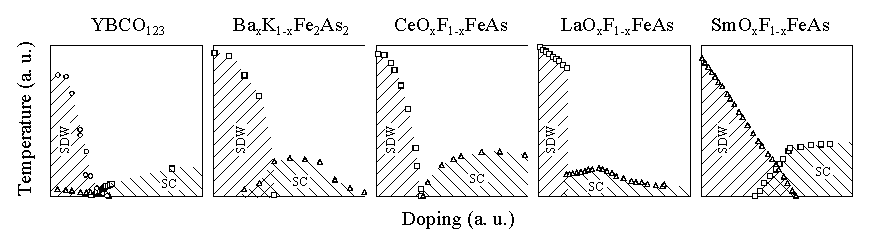
\includegraphics[scale=0.85]{Chapter-Introduction/Figures/PhaseDiagrams/PhaseDiagrams}
        \caption{Phase diagrams for various \highTc materials adapted from ref.~\cite{Uemura2009} showing the proximity of the superconducting phase (SC) to the spin density wave state (SDW) in all cases}
        \label{Fig:Theo:PhaseDiagrams}
    \end{center}
\end{figure}
As described in more detail in section~\ref{Sec:Theo:SpinDensityWave}, the \ac{SDW} state is a general form of magnetic order that describes a periodic modulation of the spins of a system and encompasses antiferromagnetism and arguably ferromagnetism. As a system enters a \ac{SDW} state, short range, damped, antiferromagnetic fluctuations occur and it is these that are thought to provide the pairing interaction for the Cooper pair states.

Spin fluctuations were originally investigated as a mechanism which \emph{suppressed} conventional, i.e. $s$-wave, superconductivity~\cite{Berk1966} from ferromagnetic fluctuations and were used to explain why nearly ferromagnetic metals such as Pd has lower than expected $T_c$. Later however it was found that for symmetries such as $d$-wave that \emph{antiferromagnetic} spin fluctuations could possibly provide an interaction which is attractive and could overcome the Coulomb repulsion~\cite{Scalapino1995}.

Typically spin-fluctuations occur due to favourable band structure conditions, in particular where there is a \emph{nesting} condition. This is where a hole-like Fermi surface band maps through reciprocal space onto a similarly sized electron-like Fermi surface via a particular vector $\vect{q}$ known as the nesting vector. Since strong nesting leads to a stable \ac{SDW} state, we are looking for only partial nesting in the Fermi surface of superconducting materials so that we get enough spin fluctuations to cause pairing but not too many to cause a full \ac{SDW} state.

As an aside, nesting is not the only cause of spin fluctuations. For example, frustrated spin systems such as the Kagome triangular lattice can also be a cause of spin fluctuations, however this is thought to occur only in very specific 1D and 2D materials.

\subsection{Pairing in the pnictides}

Soon after the discovery of the pnictide materials, a possible pairing mechanism was proposed based on on the above described spin density wave fluctuations. The original paper suggested a $s_{\pm}$ gap symmetry~\cite{Mazin2008} which features a multi band model based on LaFeAsO$_{1-x}$F$_x$. The spin fluctuation coupling vector couples over the \ac{BZ} diagonal two separate, approximately cylindrical, Fermi surfaces of opposite phase. Although this is an extended $s$-wave model, the geometry is satisfied by the relative positions of the Fermi surfaces within the \ac{BZ}. 

As already stated, more recent measurements have discovered nodes in the gap structure in many pnictide materials and while no nodes featured in the original Mazin model, there is no reason why the model can be adapted to include them.

% \TODO{What actually is the cause of the attraction in the nesting picture? ... Spin fluctuation interaction in real space is approximately proportional to the dipole interaction $V=-\mu . \mu \chi(r)$}%\cite{Bergemann2003}

% Strong correlations - the interaction energy is much greater than the kinetic energy for the states
% When correlations present, Cooper pairs are assumed to be pairs of Landau quasiparticles

% The Stoner condition of $\mathcal{N}_0 I > 1$ -- where $\mathcal{N}_0$ is the density of states at the Fermi energy and $I$ is the molecular field constant, that scales the magnetism given a field -- indicates an energy instability\cite{Kubler2000}

